%  American Nuclear Society Transaction template
%  by Diego Mandelli (INL)
%  Most of the template has been built by Seth R. Johnson
%  based on the ANS transaction guidelines

\documentclass{anstrans}

\usepackage{algorithm}
\usepackage{algpseudocode}
\usepackage{graphicx}
\usepackage{amsmath}
% \usepackage{fmtcount}

\usepackage[none]{hyphenat}

%%%%%%%%%%%%%%%%%%%%%%%%%%%%%%%%%%%
\title{PERFORMING PROBABILISTIC RISK ASSESSMENT THROUGH RAVEN}
\author{A. Alfonsi \and  C. Rabiti \and D. Mandelli \and J.J. Cogliati \and R.A. Kinoshita}

\institute{
Idaho National Laboratory
}

\email{ \{andrea.alfonsi, cristian.rabiti, diego.mandelli, joshua.cogliati, robert.kinoshita\}@inl.gov }

%%%% packages and definitions (optional)
\usepackage{graphicx} % allows inclusion of graphics
\usepackage{booktabs} % nice rules (thick lines) for tables
\usepackage{microtype} % improves typography for PDF
\usepackage{dblfloatfix} % fix two-column floats to allow bottom placement

\newcommand{\SN}{S$_N$}
\renewcommand{\vec}[1]{\bm{#1}} %vector is bold italic
\newcommand{\vd}{\bm{\cdot}} % slightly bold vector dot
\newcommand{\grad}{\vec{\nabla}} % gradient
\newcommand{\ud}{\mathop{}\!\mathrm{d}} % upright derivative symbol

\begin{document}
%%%%%%%%%%%%%%%%%%%%%%%%%%%%%%%%%%%%%%%%%%%%%%%%%%%%%%%%%%%%%%%%%%%%%%%%%%%%%%%%
  \twocolumn[
    \begin{@twocolumnfalse}
        \maketitle
    \end{@twocolumnfalse}
  ]

%%%%%%%%%%%%%%%%%%%%%%%%%%%%%%%%%%%%%%%%%%%%%%%%%%%%%%%%%%%%%%%%%%%%%%%%%%%%%%%%
\section{Introduction}
%%%%%%%%%%%%%%%%%%%%%%%%%%%%%%%%%%%%%%%%%%%%%%%%%%%%%%%%%%%%%%%%%%%%%%%%%%%%%%%%
RAVEN (\textbf{R}eactor \textbf{A}nalysis and \textbf{V}irtual control \textbf{EN}viroment)~\cite{ravenFY12,mandelliANS2012} is a software framework that acts as the control logic driver for the Thermal-Hydraulic code RELAP-7, a newly developed software at Idaho National Laboratory. This paper provide an overview of the RAVEN software structure and its utilization in conjunction with RELAP-7/MOOSE~\cite{MOOSE,relap7FY12}. RAVEN is a multi-purpose Probabilistic Risk Assessment (PRA) code that allows dispatching different functionalities.
It is designed to derive and actuate the control logic required to simulate both plant control system and operator actions (guided procedures) and to perform both Monte-Carlo sampling of random distributed events and dynamic event tree based analysis~\cite{ADAPTHakobyan}.
In order to assist the user in the input/output handling, a Graphical User Interface (GUI) and a post-processing data mining module, based on dimensionality and cardinality reduction~\cite{mandelliEsrel2011}, are available.
This paper focuses on the link between the software layout and the mathematical framework from which its structure is derived. In order to show the code capabilities, a demo of a Station Black Out (SBO) analysis of a simplified Pressurized Water Reactor (PWR) model is presented.
%%%%%%%%%%%%%%%%%%%%%%%%%%%%%%%%%%%%%%%%%%%%%%%%%%%%%%%%%%%%%%%%%%%%%%%%%%%%%%%%
\section{MATHEMATICAL FRAMEWORK}
%%%%%%%%%%%%%%%%%%%%%%%%%%%%%%%%%%%%%%%%%%%%%%%%%%%%%%%%%%%%%%%%%%%%%%%%%%%%%%%%
\label{sec:mathFramework}
Let be $\bar{\theta}(t)$ a vector describing the plant status in the phase space; the dynamic of the plant, including the control system, can be summarized by the following equation:
\begin{equation}
\frac{\partial \bar{\theta}}{\partial t} = \bar{H}(\theta(t),t)
\label{eq:SystemDynamics}
\end{equation}
In the above equation it is assumed the time differentiability in the phase space. Performing an arbitrary decomposition of the phase space, the following statement is obtained:
\begin{equation}
\bar{\theta}=\binom{\bar{x}}{\bar{v}}
\label{eq:firstDecomposition}
\end{equation}

The decomposition is made in such a way that $\bar{x}$ represents the unknowns solved by RELAP-7, while $\bar{v}$ are the variables directly controlled by the control system (i.e., RAVEN). Equation~\ref{eq:SystemDynamics} can now be rewritten as follows:
\begin{equation}
\begin{cases}
\dfrac{\partial \bar{x}}{\partial t} = \bar{F}(\bar{x},\bar{v},t) \\
\dfrac{\partial \bar{v}}{\partial t} = \bar{V}(\bar{x},\bar{v},t) \\
\end{cases}
\label{eq:generalSystemEquation}
\end{equation}
It is possible to note that the function $\bar{V}(\bar{x},\bar{v},t)$ representing the control system, does not depend on the knowledge of the complete status of the system but on a restricted subset (i.e. control variables) $\bar{C}$:
\begin{equation}
\begin{cases}
\dfrac{\partial \bar{x}}{\partial t} = \bar{F}(\bar{x},\bar{v},t) \\
\bar{C} = \bar{G}(\bar{x},t) \\
\dfrac{\partial \bar{v}}{\partial t} = \bar{V}(\bar{x},\bar{v},t)
\end{cases}
\label{eq:generalSystemEquationwithControl}
\end{equation}

The system of equations in Eq.~\ref{eq:generalSystemEquationwithControl} is fully coupled and has commonly been solved by an operator splitting approach. The reasons for this choice are several:
\begin{itemize}
\item Control system reacts with an intrinsic delay
\item The reaction of the control system might move the system between two different discrete states and
therefore numerical errors will be always of first order unless the discontinuity is treated explicitly.
\end{itemize}
\begin{figure}
\centering
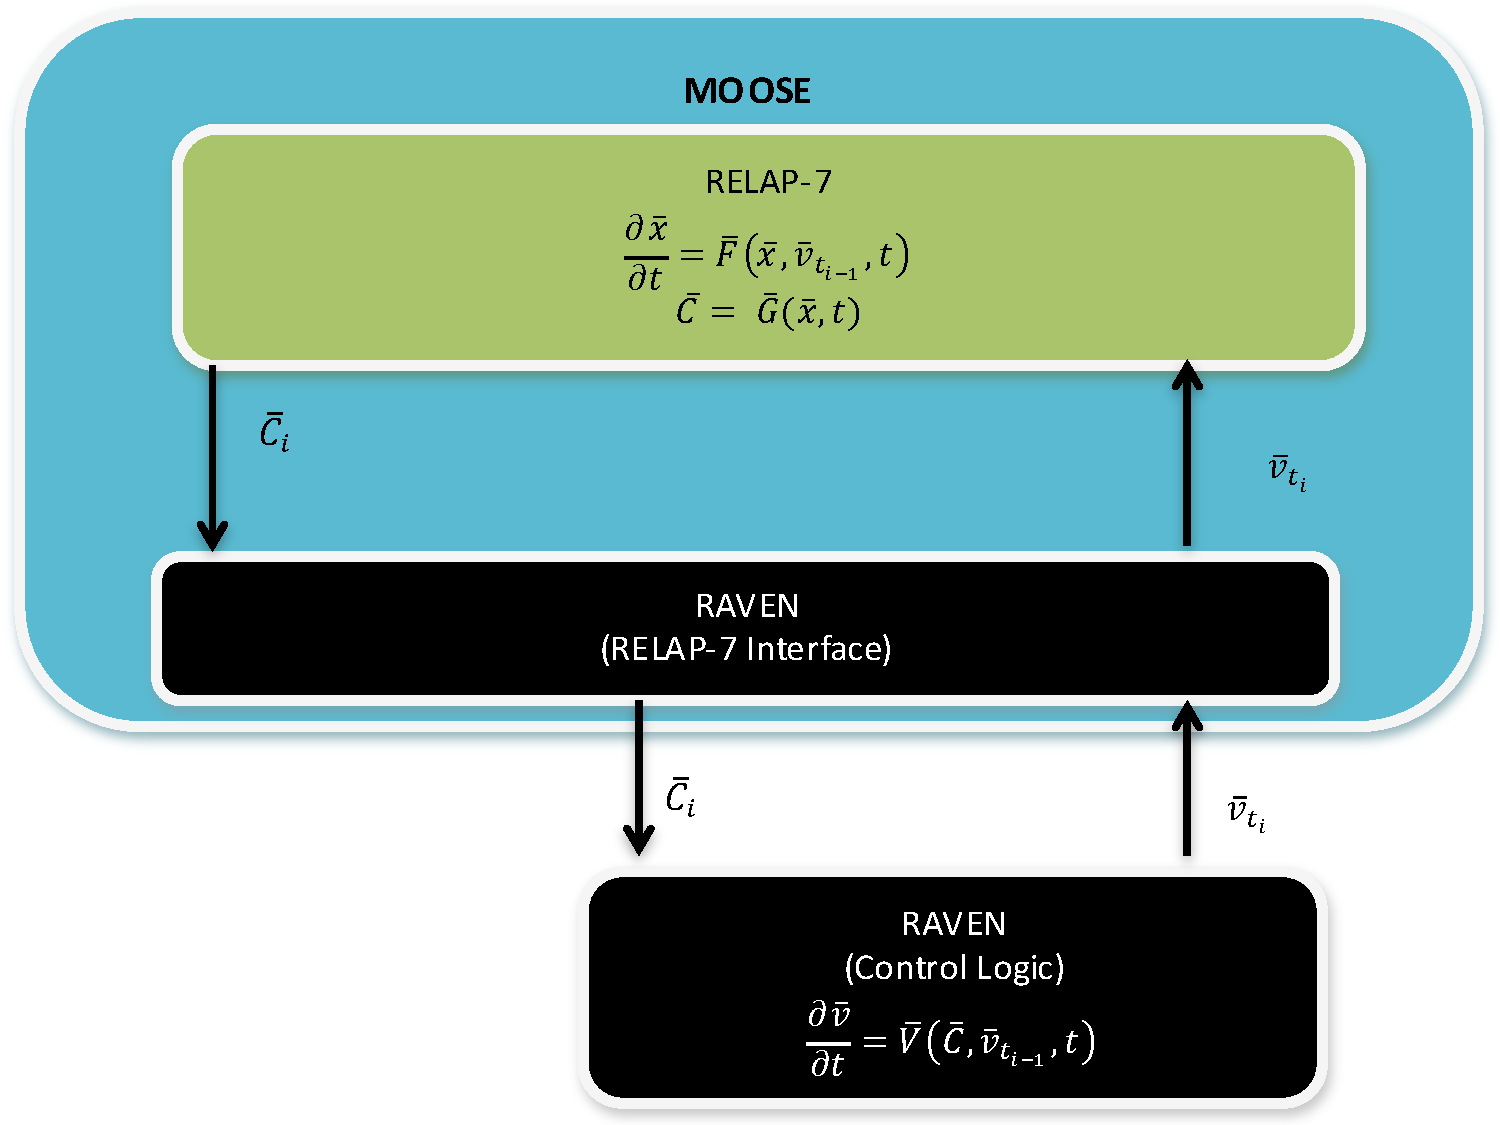
\includegraphics[width=0.35\textwidth]{figures/ControlSystemSoftwareLayout.pdf}
\caption{Control System Software Layout.}
\label{fig:ControlSoftwareLayout}
\end{figure}
Thus, RAVEN is using this approach (Fig.~\ref{fig:ControlSoftwareLayout}) to solve Eq.~\ref{eq:generalSystemEquationwithControl} which becomes:
\begin{equation}
\begin{cases}
\dfrac{\partial \bar{x}}{\partial t} = \bar{F}(\bar{x},\bar{v}_{t_{i-1}},t) \\
\bar{C} = \bar{G}(\bar{x},t) & t_{i-1}\leq t\leq t_{i} = t_{i-1} + \Delta t_{i}\\
\dfrac{\partial \bar{v}}{\partial t} = \bar{V}(\bar{x},\bar{v}_{t_{i-1}},t) \\
\end{cases}
\label{eq:generalSystemEquationwithControlSplitting}
\end{equation}
Even if all information needed is contained in $\bar{x}$ and $\bar{v}$, it is not a practical and efficient way to implement the control system. Hence, a system of auxiliary variables has been introduced.
The auxiliary variables are those that in statistical analysis are artificially added, when possible, to non-Markovian systems into the space phase to obtain a Markovian behavior back, so that only the information of the previous time step is needed to determine the future status of the system.
Thus, the introduction of the auxiliary system into the mathematical framework leads to the following formulation of the Eq.~\ref{eq:generalSystemEquationwithControlSplitting}:
\begin{equation}
\begin{cases}
\dfrac{\partial \bar{x}}{\partial t} = \bar{F}(\bar{x},\bar{v}_{t_{i-1}},t) \\
\bar{C} = \bar{G}(\bar{x},t) & t_{i-1}\leq t\leq t_{i} = t_{i-1} + \Delta t_{i}\\
\dfrac{\partial \bar{a}}{\partial t} = \bar{A}(\bar{x},\bar{C},\bar{a}_{t_{i-1}},\bar{v}_{t_{i-1}},t) \\
\dfrac{\partial \bar{v}}{\partial t} = \bar{V}(\bar{x},\bar{v}_{t_{i-1}},\bar{a},t)
\end{cases}
\label{eq:generalSystemEquationwithControlSplittingAndAux}
\end{equation}


%%%%%%%%%%%%%%%%%%%%%%%%%%%%%%%%%%%%%%%%%%%%%%%%%%%%%%%%%%%%%%%%%%%%%%%%%%%%%%%%
\section{SOFTWARE STRUCTURE}
%%%%%%%%%%%%%%%%%%%%%%%%%%%%%%%%%%%%%%%%%%%%%%%%%%%%%%%%%%%%%%%%%%%%%%%%%%%%%%%%
RAVEN, is plugged with the software environment MOOSE~\cite{MOOSE}. MOOSE is a computer simulation framework,  developed at Idaho National Laboratory (INL), that simplifies the process for predicting the behavior of complex systems and developing non-linear, multi-physics simulation tools. Other than providing the algorithms for the solution of the differential equation, MOOSE also provides all the manipulation tools for the \verb!C++! classes containing the solution vector. This framework has been used to construct and develop the Thermal-Hydraulic code RELAP-7, giving an enormous flexibility in the coupling procedure with RAVEN.

RELAP-7 is the next generation nuclear reactor system safety analysis. It will become the main reactor systems simulation toolkit for RISMC (\textbf{R}isk \textbf{I}nformed \textbf{S}afety \textbf{M}argin \textbf{C}haracterization)~\cite{mandelliANS_RISMC} project and the next generation tool in the RELAP reactor safety/systems analysis application series.
RAVEN has been developed in a high modular and pluggable way in order to enable easy integration of different programming languages (i.e., \verb!C++!, \verb!Python!) and coupling with other applications including the ones based on MOOSE. The code consists of four main modules:
\begin{itemize}
\item RAVEN/RELAP-7 interface
\item \verb!Python! Control Logic
\item \verb!Python! Calculation Driver
\item Graphical User Interface
\end{itemize}

The RAVEN/RELAP-7 interface, coded in \verb!C++!, is the container of all the tools needed to interact with RELAP-7/MOOSE. It has been designed in order to be general and pluggable with different solvers simultaneously in order to allow an easier and faster development of the control logic/PRA capabilities for multi-physics applications.
%(to properly generate the monitored quantities and accordingly modify the controlled
% parameters in the raven/relap7 simulation)
The interface provieds all the capabilities to generate the monitored quantities and accordingly modify the controlled parameters in the RELAP-7/MOOSE calculation.
%The interface provides all the capabilities to control, monitor, and process the %parameters/quantities in order to drive the RELAP-7/MOOSE calculation.
In addition, it contains the tools to communicate to the MOOSE input parser which information, i.e. input syntax, must be provided in order to run a RAVEN  calculation.\\The control logic module is used to drive a RAVEN/RELAP-7 calculation. Up to now it is implemented by the user via \verb!Python! scripting. The reason of this choice is to try to preserve generality of the approach in the initial phases of the project so that further specialization is possible and  inexpensive. The implementation of the control logic via \verb!Python! is rather convenient and flexible. The user only needs to know few \verb!Python! syntax rules in order to build an input. Although this extreme simplicity, it will be part of the GUI task to automatize the construction of the control logic scripting in order to minimize user effort.

The core of PRA analysis is contained in the module called "Raven Runner". It consists of a \verb!Python! driver in which Monte-Carlo based algorithm has been implemented. It calls RAVEN multiple times, changes initial conditions and seeds the random generator for the distributions.
The multiple calculations, required by the employment of these algorithms, can be run in parallel, using queues/sub-process/\verb!Python! systems. The analysis of dynamic stochastic systems through Monte-Carlo algorithm can be summarized as follows:
\begin{enumerate}
\item Initial Sampling of:
       \begin{enumerate}
       \item Physical parameters
       \item Initial conditions
       \item Transition conditions, i.e. time instant in which transition events occur (e.g., time in which a reactor scram occurs, etc.)
    \end{enumerate}
\item Run the system simulator using the values previously sampled and eventually applying a random noise to some parameters at each time step
\item Repeat 1 and 2 for a large number of calculations (user input)
\end{enumerate}
The "runner" basically performs a different seeding of the random number generator and interact, through RAVEN, with the \verb!Python! control logic input in order to sample the variables specified by the user.

As previously mentioned, a Graphical User Interface (GUI) is not required to run RAVEN, but it represents an added value to the whole code. The GUI is compatible with all the capabilities actually present in RAVEN (control logic, Monte-Carlo, etc.).  Its development is performed using QtPy, which is a \verb!Python! interface for a \verb!C++! based library (\verb!C++!) for GUI implementation. The GUI is based on a software named Peacock, which is a GUI interface for MOOSE based application and, in its base implementation, is only able to assist the user in the creation of the input.  In order to make it fit all the RAVEN needs, the GUI has been specialized and is in continuous evolution.
%%%%%%%%%%%%%%%%%%%%%%%%%%%%%%%%%%%%%%%%%%%%%%%%%%%%%%%%%%%%%%%%%%%%%%%%%%%%%%%%
\section{DEMO FOR A PWR PRA ANALYSIS}
%%%%%%%%%%%%%%%%%%%%%%%%%%%%%%%%%%%%%%%%%%%%%%%%%%%%%%%%%%%%%%%%%%%%%%%%%%%%%%%%
In order to show the capabilities of RAVEN coupled with RELAP-7/MOOSE, a PRA analysis on a simplified PWR model (Fig.~\ref{fig:PWRmodel}) has been employed.
\begin{figure}
   \centering
    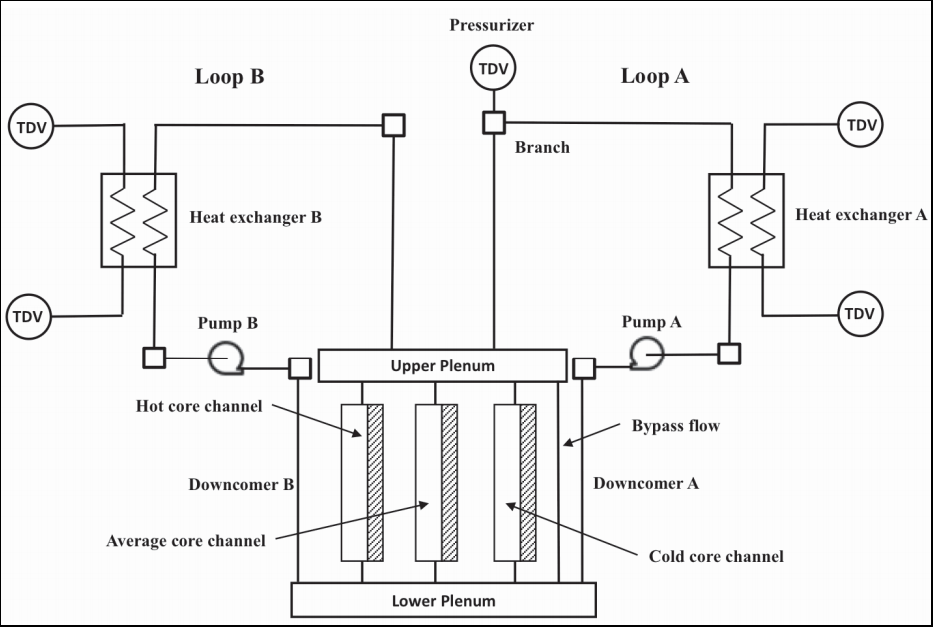
\includegraphics[width=0.4\textwidth]{figures/PWR_TMI_SCHEME.PNG}
    \caption{PWR model scheme.}
    \label{fig:PWRmodel}
\end{figure}
\\Since RELAP-7 still has limitations for the component controllable parameters and models, it has been necessary to act on unconventional factors (i.e. inlet/outlet friction factors in order to simulate a realistic pump coast-down).
\begin{figure} [H]
\centering
  \centering
  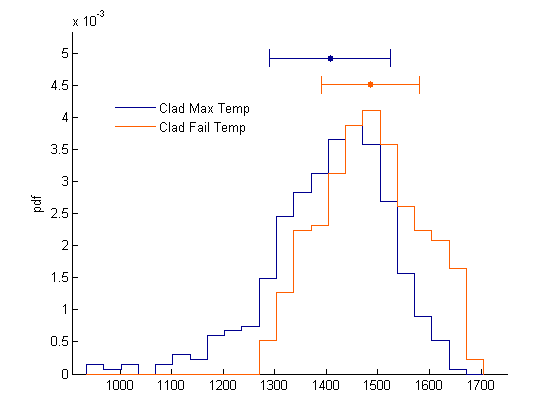
\includegraphics[width=0.35\textwidth]{figures/PRA_dist2.png}
  \label{fig:pdf_temp}
   \caption{Comparison between max reached clad temperature and clad failure temperature distributions: Probability distribution functions.}
\label{fig:distributionResults}
\end{figure}

The Probabilistic Risk Assessment analysis has been performed simulating a Station Black Out accident, running Monte-Carlo samplings (400 simulations) on the recovery time of the diesel generators $t_{1}$ (Normal distribution, mu = 120 s, sigma = 20 s) and the clad failure temperature $TC{f}$(Triangular distribution, xPeak = 1477.59 K, xMin~ =~1255.37 K, xMax = 1699.82 K). Since the scope of this demo is to show the functionalities contained in RAVEN and RELAP-7 is not yet optimized for long simulation times, the transient has been accelerated in order to simulate a maximum of 300 seconds.
Figure~\ref{fig:distributionResults} shows the distribution of the maximum temperature reached by the clad in the core channels (blue histogram) and compares it with the distribution of clad failure temperature (red histogram).
As already mentioned, the transient has been accelerated, since the scope of the analysis was just to show RAVEN capabilities to perform stochastic analysis of relatively complex systems. %That can explain the large overlapping of the two distributions, which indicates a high failure %probability of the system considered.

Figure~\ref{fig:limit_surface_rng_temp_and_dg} shows the limit surface, i.e. the boundaries between system failure (red points) and system success (green points), obtained by the 400 Monte-Carlo simulations. Since only two uncertain parameters have been considered (i.e., DG recovery time and clad fail temperature), this boundary lies in a 2-dimensional space.
The slope of the limit surface pictured in Fig.~\ref{fig:limit_surface_rng_temp_and_dg} also shows, in this particular demo, how the DG recovery time has a greater impact on the system dynamics then the clad failure temperature.
\begin{figure}
   \centering
    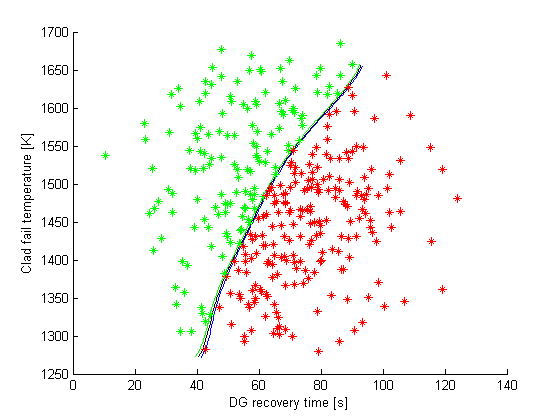
\includegraphics[width=0.45\textwidth]{figures/PRA_limitSurface.png}
    \caption{Limit Surface for the SBO analysis of a simplified PWR model}
    \label{fig:limit_surface_rng_temp_and_dg}
\end{figure}
%%%%%%%%%%%%%%%%%%%%%%%%%%%%%%%%%%%%%%%%%%%%%%%%%%%%%%%%%%%%%%%%%%%%%%%%%%%%%%%%
\section{CONCLUSIONS}
%%%%%%%%%%%%%%%%%%%%%%%%%%%%%%%%%%%%%%%%%%%%%%%%%%%%%%%%%%%%%%%%%%%%%%%%%%%%%%%%
In this paper it has been presented RAVEN as a tool to perform dynamic PRA through Monte-Carlo sampling. In particular, the software structure and all the components that are involved in the computation have been presented, including system simulator (i.e., RELAP-7) and the control logic, characterized by a monitoring system and on-line control of selected parameters.
An example of PRA analysis has been also presented for a SBO-like case for a simplified PWR loop.
The description of the implementation for such case demonstrates how the flexibility of the software framework provides the basic tools to perform Dynamic PRA, uncertainty quantification and plant control.
Next capabilities, to be implemented to RAVEN and that are currently under development, include dynamic event tree generation~\cite{ADAPTHakobyan}, adaptive sampling~\cite{mandelliSVMANS} and more advanced data mining algorithms~\cite{mandelliEsrel2011}.
%%%%%%%%%%%%%%%%%%%%%%%%%%%%%%%%%%%%%%%%%%%%%%%%%%%%%%%%%%%%%%%%%%%%%%%%%%%%%%%%
\section{ENDNOTES}
%%%%%%%%%%%%%%%%%%%%%%%%%%%%%%%%%%%%%%%%%%%%%%%%%%%%%%%%%%%%%%%%%%%%%%%%%%%%%%%%
This work is supported by the U.S. Department of Energy, under DOE Idaho Operations Office Contract DE-AC07-05ID14517. Accordingly, the U.S. Government retains a nonexclusive, royalty-free license to publish or reproduce the published form of this contribution, or allow others to do so, for U.S. Government purposes.

\bibliographystyle{ans}
\bibliography{bibl}
\end{document}

